\documentclass{sigchi}

% Use this command to override the default ACM copyright statement (e.g. for preprints). 
% Consult the conference website for the camera-ready copyright statement.


%% EXAMPLE BEGIN -- HOW TO OVERRIDE THE DEFAULT COPYRIGHT STRIP -- (July 22, 2013 - Paul Baumann)
% \toappear{Permission to make digital or hard copies of all or part of this work for personal or classroom use is 	granted without fee provided that copies are not made or distributed for profit or commercial advantage and that copies bear this notice and the full citation on the first page. Copyrights for components of this work owned by others than ACM must be honored. Abstracting with credit is permitted. To copy otherwise, or republish, to post on servers or to redistribute to lists, requires prior specific permission and/or a fee. Request permissions from permissions@acm.org. \\
% {\emph{CHI'14}}, April 26--May 1, 2014, Toronto, Canada. \\
% Copyright \copyright~2014 ACM ISBN/14/04...\$15.00. \\
% DOI string from ACM form confirmation}
%% EXAMPLE END -- HOW TO OVERRIDE THE DEFAULT COPYRIGHT STRIP -- (July 22, 2013 - Paul Baumann)


% Arabic page numbers for submission. 
% Remove this line to eliminate page numbers for the camera ready copy
% \pagenumbering{arabic}


% Load basic packages
\usepackage{balance}  % to better equalize the last page
\usepackage{graphics} % for EPS, load graphicx instead
\usepackage{times}    % comment if you want LaTeX's default font
\usepackage{url}      % llt: nicely formatted URLs
\usepackage{ntheorem}
\newtheorem{hyp}{Hypothesis} 
% llt: Define a global style for URLs, rather that the default one
\makeatletter
\def\url@leostyle{%
  \@ifundefined{selectfont}{\def\UrlFont{\sf}}{\def\UrlFont{\small\bf\ttfamily}}}
\makeatother
\urlstyle{leo}


% To make various LaTeX processors do the right thing with page size.
\def\pprw{8.5in}
\def\pprh{11in}
\special{papersize=\pprw,\pprh}
\setlength{\paperwidth}{\pprw}
\setlength{\paperheight}{\pprh}
\setlength{\pdfpagewidth}{\pprw}
\setlength{\pdfpageheight}{\pprh}

% Make sure hyperref comes last of your loaded packages, 
% to give it a fighting chance of not being over-written, 
% since its job is to redefine many LaTeX commands.
\usepackage[pdftex]{hyperref}
\hypersetup{
pdftitle={SIGCHI Conference Proceedings Format},
pdfauthor={LaTeX},
pdfkeywords={SIGCHI, proceedings, archival format},
bookmarksnumbered,
pdfstartview={FitH},
colorlinks,
citecolor=black,
filecolor=black,
linkcolor=black,
urlcolor=black,
breaklinks=true,
}

% create a shortcut to typeset table headings
\newcommand\tabhead[1]{\small\textbf{#1}}


% End of preamble. Here it comes the document.
\begin{document}

\title{Using Leap Motion to Improve ASL Learning}

\numberofauthors{3}
\author{
  \alignauthor Manni Gong\\
    \affaddr{Affiliation}\\
    \email{e-mail address}\\
  \alignauthor Minshan Tao\\
    \affaddr{Affiliation}\\
  \alignauthor Zach Welch\\
    \affaddr{Department of Computer Sciences}\\
    \email{zwelch@cs.wisc.edu}\\
}

\maketitle

\begin{abstract}
Teaching American Sign Language (ASL) can be a difficult, time consuming task. A popular aid in ASL learning has been visual feedback, as from a video camera. New technological developments in motion tracking, like the Microsoft Kinect and the Leap Motion hand tracker, provide new ways to track and visualize motor functions. This paper details a study investigating the effect of automated and interactive feedback provided by Leap Motion on recall of ASL. We conducted a two-by-two between participants  study(Leap Motion: Present vs Absent; Video Feedback: Present vs Absent) in which participants were presented a series of simple ASL signs, which they were later tested on. Results show Leap F=1.376(Pr= 0.2708) and Video F=5.938 (Pr= 0.0376), which means Leap Motion has no significant effect on assisting ASL learning, but video does. Future directions and a number of improvements for Leap Motion are also discussed. 
\end{abstract}

\keywords{
	Guides; instructions; author's kit; conference publications;
	keywords should be separated by a semi-colon. \newline
	\textcolor{red}{Optional section to be included in your final version, 
  but strongly encouraged.}
}

\category{H.5.m.}{Information Interfaces and Presentation (e.g. HCI)}{Miscellaneous}

See: \url{http://www.acm.org/about/class/1998/}
for more information and the full list of ACM classifiers
and descriptors. \newline
\textcolor{red}{Optional section to be included in your final version, 
but strongly encouraged. On the submission page only the classifiers’ 
letter-number combination will need to be entered.}

\section{Introduction}
Learning sign language can be quite challenging for audibly-based speakers to learn.  As opposed to learning another spoken language, where speakers are learning new combinations of sounds to produce the same meaning, sign language represents an entirely different mode of communication.  Sign language is fundamentally a visual language rather than an auditory language.  The most commonly used form of sign language in the United States is, as the name suggests, American Sign Language. 

American Sign Language, ASL for short, is interesting because it does not attempt to be a direct translation of English in which there is a sign for each letter and words and sentences are merely spelled out as in written language.  Instead, ASL gives individual gestures word and phrase level meanings; these gestures are used to generate speech.  Proficient ASL signers can converse naturally with somewhat surprising speed.  Just as in spoken language, long pauses in which one person takes a long time to formulate a response can make communication difficult.  

Since ASL is such a visually based language, visual aids are a common tool employed when learning ASL.  These visual aids come in a variety of forms, from instructional videos of signing to watching an instructor sign to watching yourself sign in a mirror or webcam.  In particular, using a webcam can be helpful because it provides instant visual feedback as to what a person’s attempt to sign actually looks like. 

\begin{figure}
\centering
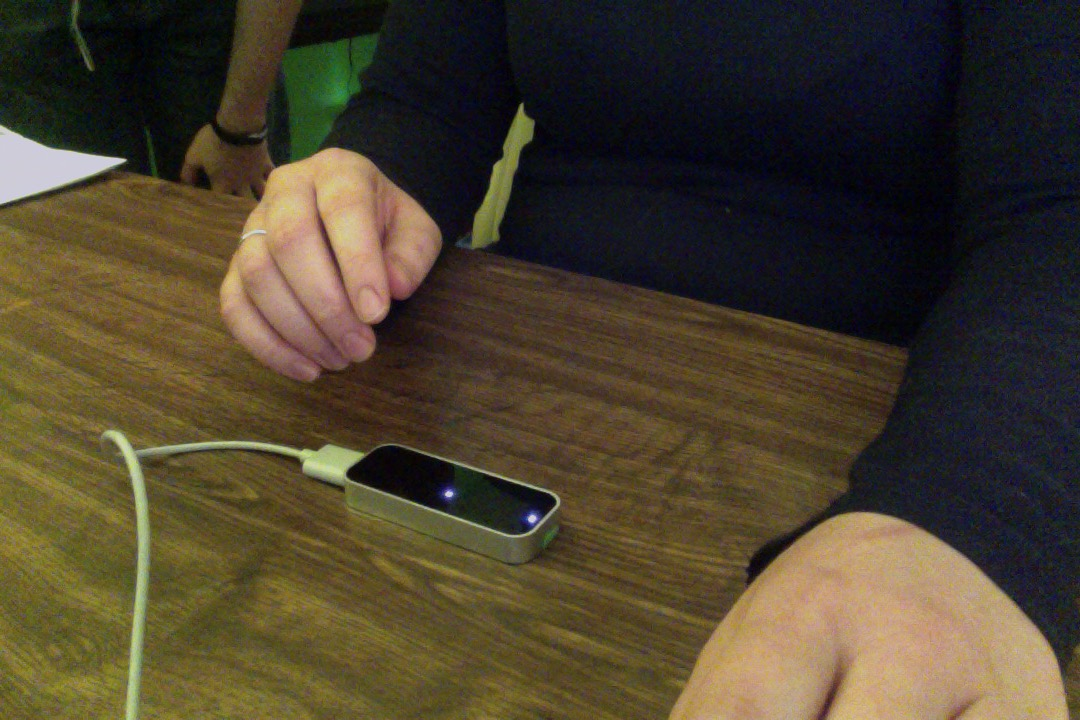
\includegraphics[width=0.5\textwidth]{leapUse.jpg}
\caption{Leap Motion ASL Tool}
\label{leapUse}
\end{figure}

New technologies like Microsoft Kinect and Leap Motion provide new ways of visualizing and interacting with physical movement.  These tools have been extensively used in games, education, and gesture based control systems.  While the Kinect is designed for full body motion tracking, and does not have much support for fine grained modeling of fingers and hands, the Leap Motion is designed specifically for tracking and modeling hands and fingers.  The Leap Motion, which can be seen in Figure ~\ref{leapUse}, is a small device which sits on a table.  When it detects hands above the device, it tracks them; this tracking data can be visualized or used as a form of input for control. There are potential issues with Leap Motion; it struggles to maintain a consistent model when the palm is perpendicular to the face of the device, as well as when there is some level of occlusion.  Additionally, when two fingers are pressed together, the Leap Motion can incorrectly report each of the finger locations. This is to be expected; Leap Motion is a new technology that is in the midst of heavy iteration by it’s design team.  Despite these issues, we believe the relatively fine grained level of tracking and modeling provided by  Leap Motion represents an exciting new potential for interactive feedback when learning ASL.  This paper describes a study to test whether the added interactivity provided by Leap Motion provides a statistically significant benefit over more traditional means of video feedback.       

\section{Background}
\subsection{Technology and Sign Language}

\subsection{Leap Motion}


\section{Hypothesis}
A relatively simple solution to give individuals learning sign language feedback is to provide them with a webcam, or even a mirror, so they can see their hands do the sign.  Leap Motion provides a potential advantage over video feedback in the area of visualizing and understanding the desired sign. While video can only show an individual their hand from a single angle, Leap Motion creates a three dimensional model of the hand that can be viewed from any angle.  Leap Motion can also provide instructors a means of recording their own interactions with Leap Motion, which the students can play back and inspect in three dimensions.  At least conceptually, this interactive medium seems to provide students a potentially valuable means of inspecting and interacting with the ASL signs.  Additionally, having interactive feedback from Leap Motion does not preclude feedback from a video feed.  This line of thinking leads to our hypothesis: 

\begin{hyp}
Individuals who receive both video feedback from a webcam and automated feedback from Leap Motion will retain information more accurately and faster compared to participants who do not receive any feedback when learning  American Sign language.
\end{hyp}

\begin{hyp}
Participants who receive both video and automated feedback will retain information more accurately and faster compared to participants who only receive one type of feedback. 
\end{hyp}

\begin{hyp}
 Participants who receive automated feedback will retain information more accurately and faster compared to participants who receive video feedback.  
\end{hyp}

\begin{hyp}
 Participants who receive either video or automated feedback will retain information more accurately and faster compared to participants who do not receive any type of feedback.
\end{hyp}

\section{Methods}
To test our hypothesis, we designed an experiment that would allow participants to interact with various methods of feedback during the learning process.  Participants would be presented a series of short recordings of a sign language instructor presenting an ASL sign.  Participants then have one minute to practice the sign with some level of feedback. After a short break, the participant’s recall speed and correctness of these signs were then tested. We recorded all testing sessions for post-experiment analysis.   
 
\subsection{Participants}

We recruited 12 participants (4 male, 8 female) to participate in our experiment. Participants were recruited from around the University of Wisconsin–Madison campus; these individuals were mostly friends and fellow graduate students. Participant ages ranged from 20 to 34, with an average age of 24.08.  None of the participants had notable previous experience with American Sign Language, which we held as a prerequisite for taking part in our study. Native and non-native English speakers were both represented in the participant group.  All participants went through the roughly thirty minute experiment; they were compensated with the authors' undying gratitude.  




\subsection{Study Design}
We designed a two-by-two (Leap Motion: present vs absent; Video Feedback: present vs absent) between-participants laboratory study to test the effectiveness of Leap Motion and Video Feedback when learning ASL.  

Each of the four combinations of independent variables represent a potential learning setting for an ASL learner.  Participants in which Leap Motion and Video are abset represent our base case, and should allow us to understand the effectiveness of each form of feedback as compared to no feedback.  We will also provide a group of participants with both Video and Leap Motion feedback, to study whether the benefits from feedback provided by each technology are cumulative.  We believe this form of study should allow us to comprehensively test the effectiveness of each form of feedback.  We prefered this model over a within participants design because we had significant concerns about the holdover effects of a single participant being exposed to the same material multiple times.  We expect the participants would universally score better on later rounds of testing, regardless of the ordering of feedback settings.  Our between participants design does mean our results will inherently contain more variability; we discuss this in greater detail later in the paper.  



  
\subsection{Task}
Prior to beginning each trial, participants were introduced to the feedback mechanisms that have been randomly selected for them. Participants were given a short window in which to get familiar with the Leap Motion interface, adjust their camera, and otherwise prepare beforehand. The participants’ goal is to watch a tutorial video of an instructor demonstrating 14 ASL signs; these signs were: Again,Hurt,  Maybe, No, Play, Same, Sign, They, What, Yes, Book, Hurry, Happy, Excuse Me.  After each sign demonstration, the participants  have 1 min to practice the sign they just learned with the provided feedback mechanism. Once all signs have been presented, the participants will watch a 10-min distraction video made up of popular clips from YouTube.  After this video, participants were given a test in which they were presented the signs they had just learned in a different order and expected to demonstrate the sign as quickly as possible.  

\subsection{Setup}

The video shown to participants was created by combining a series of short ASL instructional videos, each showing a single sign.  These individual videos were separated by 1 minute long interstitials directing the participant to practice the specific sign.  This video also contained a ten minute distraction video meant to add some distance between the learning of the signs and testing them.  This video can be viewed at http://goo.gl/uyc6RS.  

Leap Motion provides a simple Visualizer as part of it's installation which allows users to see the model of their hands as it moves according to Leap Motion. The Visualizer also contains a rudimentary camera which allows users move their viewport through space and inspect their hand motions from different angles.  While this setup may be enough to provide users with some level of feedback, we endeavored to provide an additional degree of feedback to the user.  Our initial plan was to provide users with a numerical score based on angluar differences from a reference sign motion.  In execution, we found such a model too unforgiving and difficult to get valuable improvements when using.  We then pivoted to a more visual form of feedback, one in which users could see a "ghost hand" perform the motion and attempt to line their hand motions up with the ghost hand.  This would allow users visual feedback and would allow them to easily copy cat the general motions of a sign without forcing them towards a strict standard.  Due to the limitations of Leap Motion and our hesitence do dive completely into a full fledged game engine, Leap Motion can only have one pair of hands in frame at a time.  Our final implementation plays a recording of the desired hand motion when the Leap Motion does not detect any hands in it's frame, as can be seen in Figure ~\ref{demo} in which the again sign is being shown.  The goal is to allow users the oppurtunity to watch the motion from any angle as it is supposed to occur.  When they feel confident, they can take over the hands in the frame by placing their hands over the Leap Motion.  They can try for themselves and restart the recorded ASL motion simply by removing their actual hand from over the Leap Motion.  We recorded all Leap Motion ASL recordings using a separate Leap Motion application which records hand motions into a json file. Our Leap Motion tool uses Leap Motion's LeapJS interface and should be accessable through browsers at http://pages.cs.wisc.edu/~zwelch/leap/.

To provide some users with visual feedback from a webcam, the Mac OS X Photo Booth was open during the test for some participants to use and inspect as they performed their test. Photo Booth was also used to film the testing portion of each experiment.


\begin{figure}
\centering
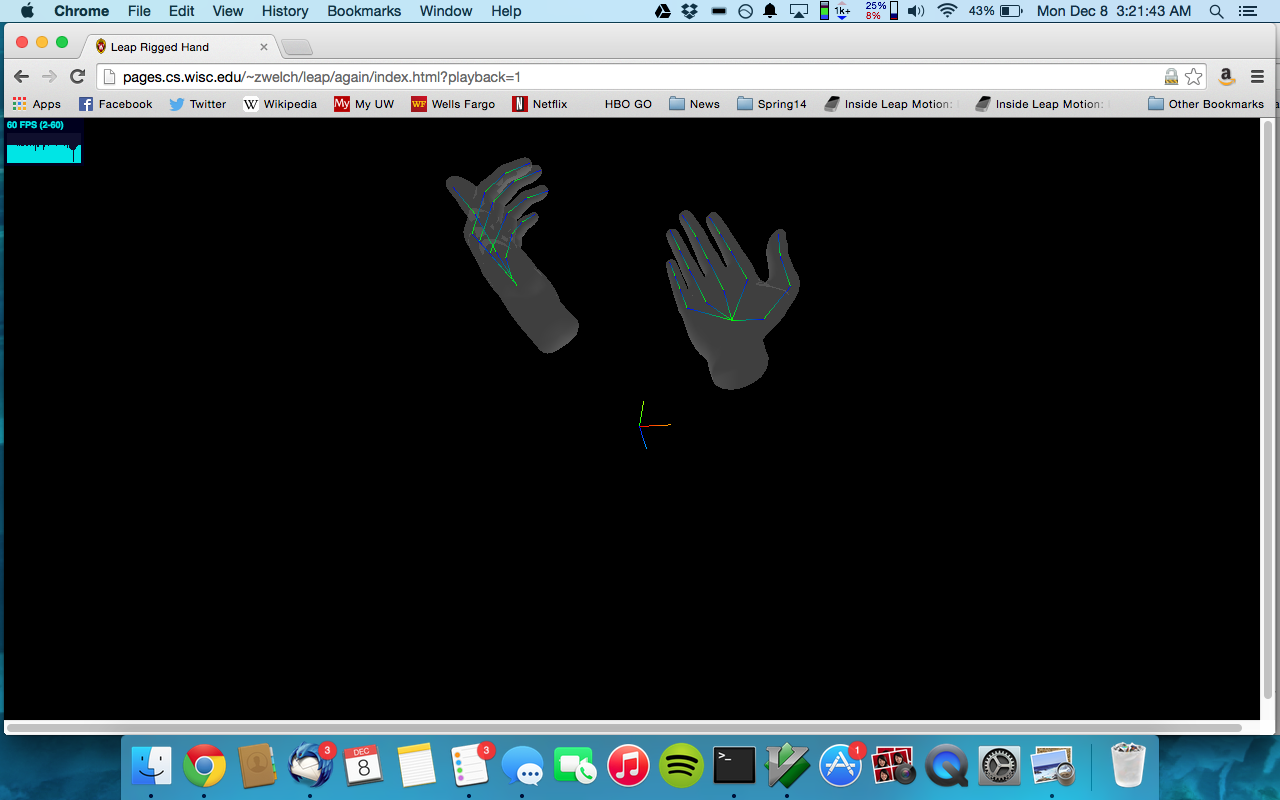
\includegraphics[width=0.5\textwidth]{demo.png}
\caption{Leap Motion ASL Tool}
\label{demo}
\end{figure}




\subsection{Procedure}
Tests were conducted in a graduate student office in CS.  Participant’s were provided with a Macbook Pro connected to a larger monitor, on which the instructional video, our Leap Motion web interface, and an instance of Photo Booth all fit comfortably.  Participants were randomly assigned a feedback setting, which they were given several minutes to familiarize themselves.  The proctor would then begin the instructional video.  The proctor remained in a corner of the room out of the Participant’s line of sight to answer questions, provide technical support, and observe the participant.  After the instructional video and ten minute distraction video, the proctor closed the instructional video and if applicable shut down the Leap Motion.  The proctor then allowed the participant to adjust the webcam before launching a Photo Booth recording (several participants did not want their face recorded, which we obliged).  A list of signs was read to each participant, with the expectation that the participant would perform the sign as quickly as possible once hearing the word.  Participant’s were allowed to pass on signs they could not remember.  

\subsection{Measures}

To measure the effectiveness of the types and combinations of feedback on a participant’s ability to recall ASL signs, we took into account two measures for each tested sign: the speed at which the participant responded and the accuracy of their sign.  The thinking here is that responsiveness and accuracy are equally important qualities for an ASL speaker to possess.  In post-experiment analysis, we studied the recorded testing session from each participant; for each sign we recorded whether 1) if the sign was correct and 2) if the participant signed within three seconds of being presented the word.  Three seconds may seem like an arbitrary time, but in practice we found that all our participants responded immediately or took a much longer time to respond.  For each sign we assigned a value of 0.5 for correctness and 0.5 for responsiveness, giving each sign a score of 0.0, 0.5, or 1.0.  We then created a final score for each participant which is the average of the score of every sign.  This overall user score was used in analysis.  

\subsection{Results}
Overall, our results find that participants performed quite well on the testing portion of our study, (M=0.801, SD=0.14), with three participants scoring a maximum score of 1.0.  The minimum score was 0.607.  The distribution of scores can be found in Figure ~\ref{boxplot}.  When we break down the results into their various factors, we find that participants with no forms of feedback performed much poorer than the average might indicate(M=0.61, SD=0.18).  Participants with the automated feedback of Leap Motion fared better, (M=0.73,  SD=0.08) but somewhat dishearteningly averaged below the overall mean.  Participants with video feedback performed slightly above average (M=0.83, SD=0.18).  Finally, participants with access to both a webcam and Leap Motion performed the best of all groups (M=0.87, SD=0.23).  According to our results, the easiest signs, which all participants received full points for, are ``Play'', ``What'', ``Book'', and ``Yes''.  The most difficult signs, both of which had a mean score of 0.458, were ``Happy'' and ``Same''.  



\begin{figure}
\centering
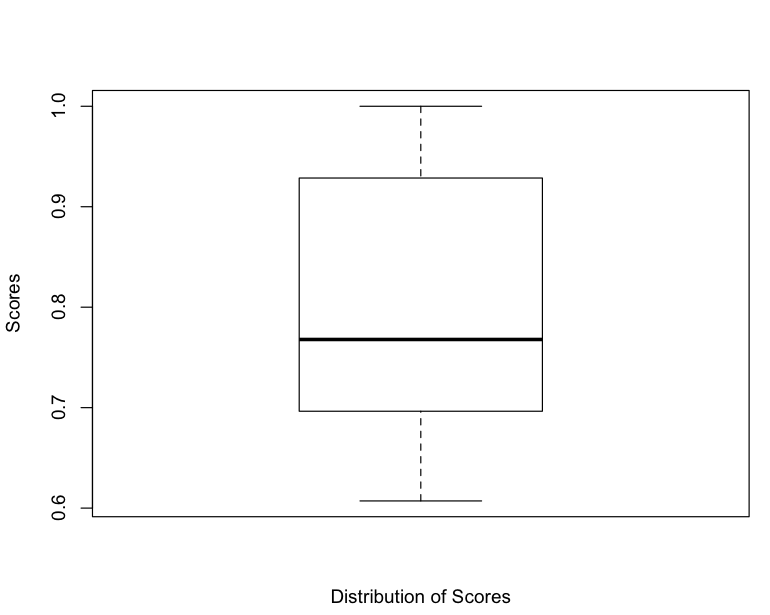
\includegraphics[width=0.4\textwidth]{boxplot.png}
\caption{Spread of Participant Scores}
\label{boxplot}
\end{figure}

We performed a two-way analysis of variance (ANOVA) with the presence of Leap and Video as input variables and participant score as a response variable.  After simplifying the model to remove a negligent interaction effect between Leap Motion and Video, we found the presence of Video has a significant effect on participant score F(1,9) = 5.938, p=0.0376.  We found no effect of the presence of Leap Motion on participant score F(1,9)=1.376, p=0.2708.  Results can be seen in Figures ~\ref{leapANOVA} and ~\ref{videoANOVA}.  There seem to be little interaction effects in our results, which can be seen in Figures ~\ref{int1} and ~\ref{int2}.

\begin{figure}
\centering
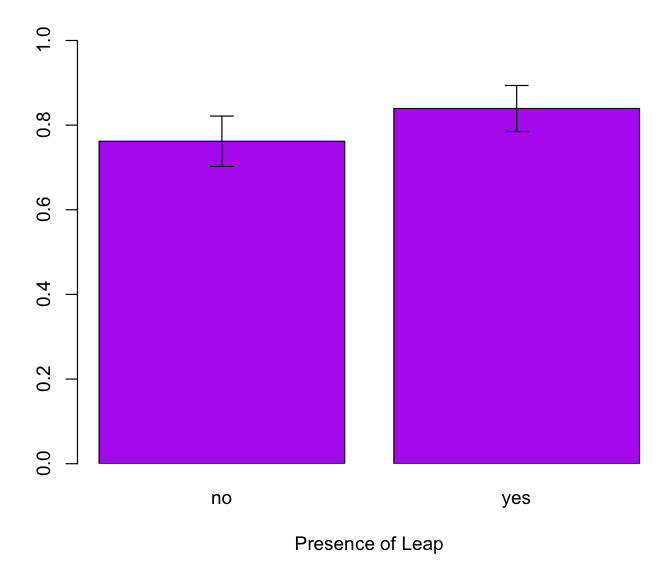
\includegraphics[width=0.4\textwidth]{leapANOVA.png}
\caption{Leap Motion Results}
\label{leapANOVA}
\end{figure}

\begin{figure}
\centering
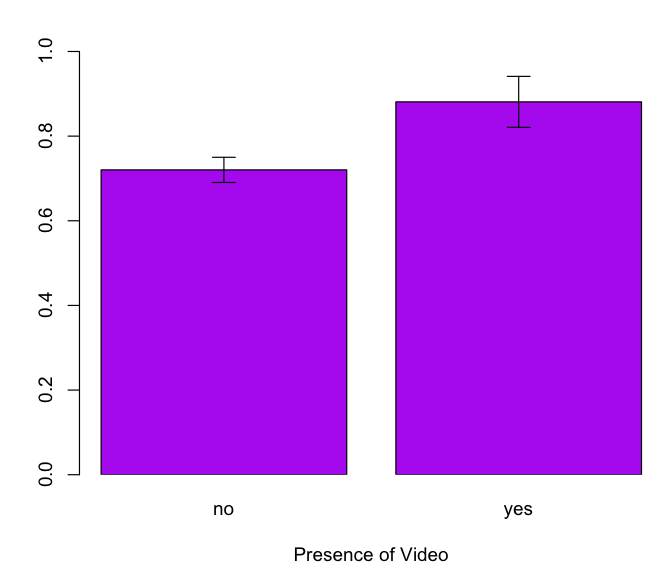
\includegraphics[width=0.4\textwidth]{videoANOVA.png}
\caption{Video Results}
\label{videoANOVA}
\end{figure}
\begin{figure}
\centering
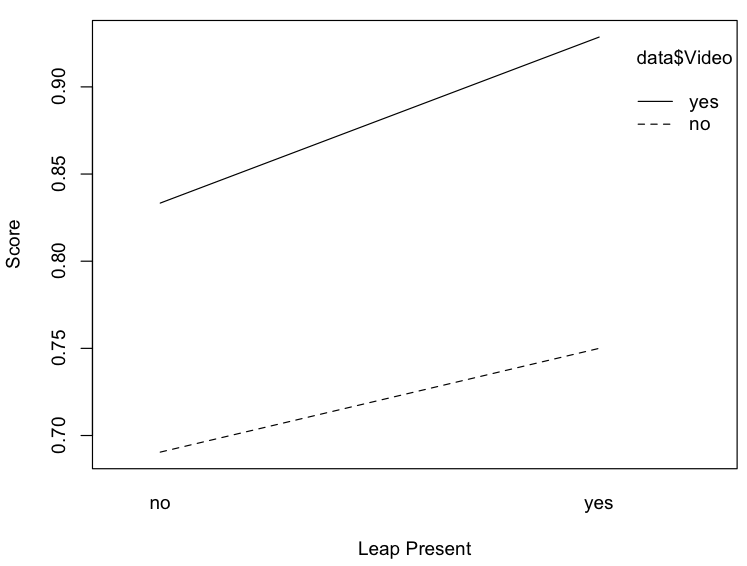
\includegraphics[width=0.25\textwidth]{int1.png}
\caption{Leap Motion Results}
\label{int1}
\end{figure}

\begin{figure}
\centering
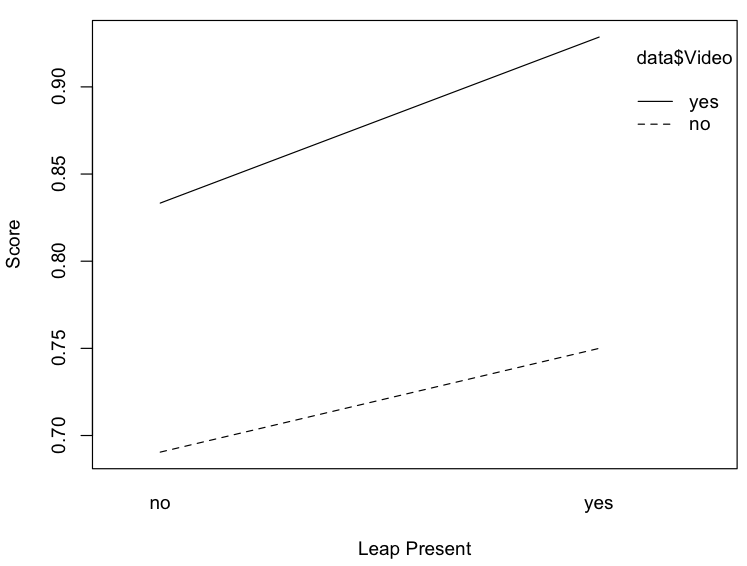
\includegraphics[width=0.25\textwidth]{int1.png}
\caption{Video Results}
\label{int2}
\end{figure}

\section{Discussion}

Though we did not hold a formal survey after the experiment to guage participant reaction to the Leap Motion, the anecdotal response of essentially all participants interacting with the Leap Motion was negative.  During the course of the Learning phase, we received questions such as "Why is it saying my hand is upside down?", "Is it broken?", and "Do I have to use this thing?".  One participant's results had to be abandoned because the Leap Motion essentially stopped working and the testing computer became unresponsive during the course of her trial.  

Our results indicate that there seems to be no benefit to using both Leap Motion and Video feedback.  Our observations during data collection may provide a possibility.  During testing, all participants provided with both forms of feedback seemed to choose a form of feedback and use only that feedback for the duration of the test. 

\section{Conclusion}



\section{Acknowledgments}
We would like to thank Dr. Mutlu for all his help along the way developing this project, as well as our participants, who made time in their schedules to be experimented on.

% Balancing columns in a ref list is a bit of a pain because you
% either use a hack like flushend or balance, or manually insert
% a column break.  http://www.tex.ac.uk/cgi-bin/texfaq2html?label=balance
% multicols doesn't work because we're already in two-column mode,
% and flushend isn't awesome, so I choose balance.  See this
% for more info: http://cs.brown.edu/system/software/latex/doc/balance.pdf
%
% Note that in a perfect world balance wants to be in the first
% column of the last page.
%
% If balance doesn't work for you, you can remove that and
% hard-code a column break into the bbl file right before you
% submit:
%
% http://stackoverflow.com/questions/2149854/how-to-manually-equalize-columns-
% in-an-ieee-paper-if-using-bibtex
%
% Or, just remove \balance and give up on balancing the last page.
%
\balance

\bibliographystyle{acm-sigchi}
\bibliography{paper}
\end{document}














